\documentclass[12pt,a4paper,titlepage]{scrartcl}

\usepackage{comment}
\usepackage[main=ngerman,english]{babel}
\usepackage[utf8]{inputenc}
\usepackage[T1]{fontenc}
\usepackage{lmodern}
\usepackage{geometry}
\geometry{left=2.5cm,right=2.5cm,top=2.5cm,bottom=3cm,head=29pt,foot=25pt}
\setlength{\footheight}{25pt}
\usepackage{microtype}
\usepackage{amsmath,amssymb,mathtools}
\numberwithin{equation}{section}
\numberwithin{table}{section}
\numberwithin{figure}{section}
\usepackage{siunitx}
\sisetup{locale=DE, separate-uncertainty=true, per-mode=fraction}
\usepackage{booktabs}
\usepackage{multirow}
\usepackage{graphicx}
\usepackage{float}
\usepackage{caption}
\usepackage{subcaption}
\usepackage[automark]{scrlayer-scrpage}
\usepackage[most]{tcolorbox}
\usepackage{hyperref}
\usepackage{pdfpages}
\usepackage{csvsimple-l3}
\usepackage{longtable}
\usepackage{graphicx}

\input{../../jupyterpackages.tex}

% jupyter nbconvert --to latex 'Path'
% enferne usepackages und begin{document} und end{document}
% \input in main.tex mit \input{Path}


\newcommand{\pdfabbildung}[2]{%
    \refstepcounter{figure}%
    \addcontentsline{lof}{figure}{\protect\numberline{\thefigure}#1}%
    \label{#2}%
}

\newcommand{\pdftabelle}[2]{%
    \refstepcounter{table}%
    \addcontentsline{lot}{table}{\protect\numberline{\thetable}#1}%
    \label{#2}%
}


\hypersetup{colorlinks=true, linkcolor=blue!60!black, urlcolor=blue!60!black, citecolor=blue!60!black}

\clearpairofpagestyles

\chead{%
    \versuch\hfill\autor\\
    \rule{\textwidth}{0.2pt}%
}
\cfoot{%
    \rule{\textwidth}{0.2pt}\\[-0.5ex]
    \pagemark\ 
}
\addtokomafont{pagefoot}{\small}
\setlength{\parindent}{0pt}

\newtcolorbox{resultbox}[1][]{ 
    enhanced,
    colback=black!4!white,
    colframe=black!65!black,
    boxrule=0.8pt,
    arc=0.0mm,
    title=#1,
    fonttitle=\bfseries,
    %drop shadow
}


\newcommand{\versuch}{Versuch 31}
\newcommand{\titel}{Optische Abbildung}
\newcommand{\praktikum}{Physikalisches Anfängerpraktikum 1}
\newcommand{\autor}{Jonathan Gießen}
\newcommand{\gruppe}{Gruppe 8}
\newcommand{\datum}{8. September 2026}
\newcommand{\betreuer}{Elias Gruber}

\begin{document}

\pagestyle{scrheadings}

\begin{titlepage}



    \centering
    \vspace*{4cm}
    {\large Universität Heidelberg\par}
    {\small Fakultät für Physik und Astronomie\par}
    {\Large \praktikum\par}
    \vspace{0.8cm}
    {\LARGE \bfseries \versuch\ -- \titel\par}
    \vspace{1.5cm}

    \begin{tabular}{ll}
        \textbf{Autor:} & \autor\\
        \textbf{Gruppe:} & \gruppe\\
        \textbf{Betreuer:} & \betreuer\\
        \textbf{Versuchsdatum:} & \datum\\
    \end{tabular}

    \vfill
    \hrulefill\
\end{titlepage}

\tableofcontents

\bigskip
\begin{tcolorbox}[colback=gray!5,colframe=gray!60,boxrule=0.8pt,arc=0.01mm,title=KI-Hinweis]
    Für die sprachliche Formulierung dieses Protokolls wurde in der Einleitung \ref{sec:einleitung} KI-gestützte Textgenerierung verwendet. 
\end{tcolorbox}


\clearpage
\section{Einleitung}\label{sec:einleitung}
Der Versuch 31 „Optische Abbildung“ behandelt die fundamentalen Prinzipien der geometrischen Optik sowie die physikalischen Grenzen optischer Instrumente, die durch wellenoptische Effekte bedingt sind. Im Zentrum des Experiments steht die Untersuchung der Bildentstehung durch die Brechung von Lichtbündeln an sphärischen Linsen, mit deren Hilfe sich reelle und virtuelle Bilder erzeugen lassen.  Ein zentraler Parameter abbildender Systeme ist die Brennweite, welche den Zusammenhang zwischen Gegenstands- und Bildweite über die optische Abbildungsgleichung beschreibt. Um die Brennweite einer Sammellinse präzise zu messen und Messfehler durch unscharfe Definitionen der Hauptebenen zu umgehen, wird im Versuch unter anderem das Bessel-Verfahren angewendet. Da reale dicke Linsen von der idealen paraxialen Näherung abweichen, ist ein weiterer Bestandteil des Versuchs die Untersuchung von typischen Abbildungsfehlern. Hierzu zählen die sphärische Aberration, bei der achsenferne Strahlen nicht in denselben Brennpunkt gelangen, sowie die chromatische Aberration, welche durch die wellenlängenabhängige Dispersion des Linsenmaterials verursacht wird.  Aufbauend auf den Eigenschaften einzelner Linsen wird im letzten Teil des Versuchs die Funktionsweise komplexerer optischer Instrumente erarbeitet, indem ein vollständiges Mikroskop aus Objektiv und Okular auf einer optischen Bank konstruiert wird. Abschließend wird das Auflösungsvermögen dieses Systems experimentell analysiert. Obwohl die Vergrößerung theoretisch durch die Wahl entsprechender Linsenbrennweiten und Tubuslängen stark gesteigert werden könnte, ist das nutzbare Auflösungsvermögen in der Realität durch die Beugung des Lichts (beschrieben durch das Rayleigh-Kriterium) physikalisch limitiert. Ziel des Versuchs ist es, diese geometrischen Gesetzmäßigkeiten der Abbildung zu überprüfen, Linsenfehler zu quantifizieren und die wellenoptischen Grenzen des Auflösungsvermögens nachzuvollziehen.

\section{Grundlagen und Theorie}

\subsection{Reelle und virtuelle Bilder sowie geometrische Abbildung}
Bei der optischen Abbildung werden Lichtbündel, die von einem Objektpunkt ausgehen, durch optische Systeme (wie Spiegel oder Linsen) so gebrochen oder reflektiert, dass sie sich in einem Bildpunkt wieder vereinigen. Dabei werden zwei Arten von Bildern unterschieden:
\begin{itemize}
    \item Reelle Bilder entstehen im tatsächlichen Schnittpunkt der Lichtbündel und können auf einem Schirm aufgefangen werden, was beispielsweise bei sphärischen Hohlspiegeln oder Sammellinsen der Fall ist.
    \item Virtuelle Bilder (wie beim Planspiegel) entstehen im Schnittpunkt der rückwärtigen Verlängerungen divergenter Lichtbündel und lassen sich nicht auf einer Mattscheibe abbilden.
\end{itemize}

Die Bildkonstruktion durch Linsen erfolgt in der sogenannten paraxialen (Gaußschen) Näherung über drei charakteristische Lichtstrahlen: 
\begin{itemize}
    \item Mittelpunktsstrahlen fallen senkrecht ein und passieren das Linsenzentrum ohne Ablenkung.
    \item Gegenstandsseitige Parallelstrahlen werden durch die Linse zu bildseitigen Brennpunktstrahlen gebrochen.
    \item Gegenstandsseitige Brennpunktstrahlen werden zu bildseitigen Parallelstrahlen abgelenkt.
\end{itemize}

Mathematisch wird dieser Zusammenhang bei dünnen Linsen durch die Abbildungsgleichung 
\begin{equation}
    \frac{1}{f} = \frac{1}{g} + \frac{1}{b}\label{eq:Linsengleichung}
\end{equation}
beschrieben, welche die Brennweite $f$ mit der Gegenstandsweite $g$ und der Bildweite $b$ verknüpft. Das Verhältnis von Bild- zu Gegenstandsgröße entspricht dabei dem Abbildungsmaßstab:
\begin{equation}
    \beta = \frac{B}{G} = \frac{b}{g}\label{eq:Verhältnis}
\end{equation}
\begin{figure}[H]
    \centering
    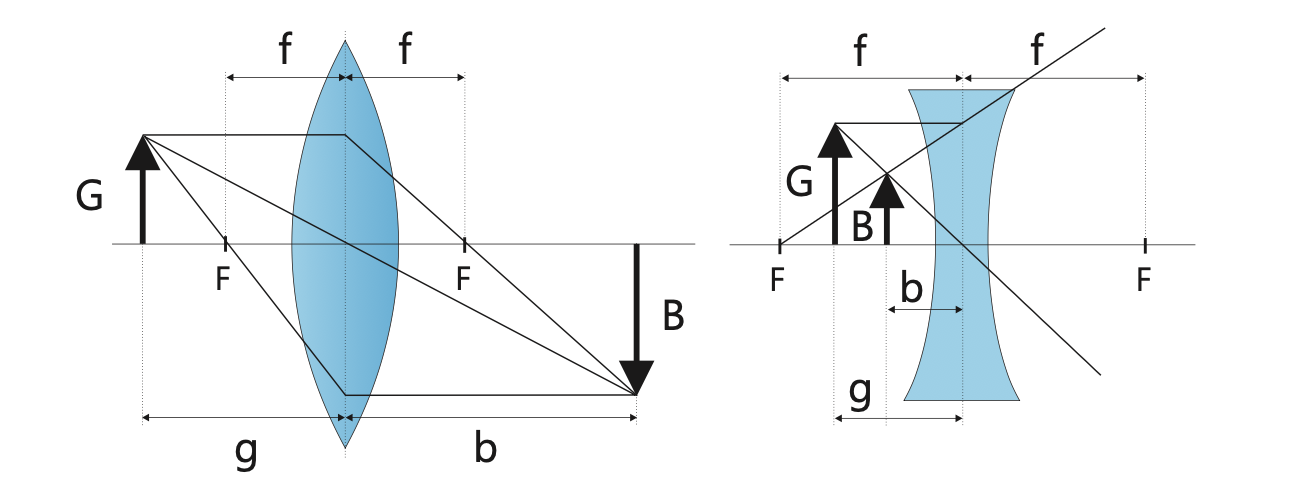
\includegraphics[width=0.6\textwidth]{img/Linsengleichung.png}
    \caption{Strahlengang druch linsen mit den charakteristischen Strahlen.}
    \label{fig:abbildung}
\end{figure}

\subsection{Brennweitenbestimmung nach Bessel}
Die direkte Messung von Bild- und Gegenstandsweite ist fehleranfällig, da sich diese Abstände bei dicken Linsen nicht auf die Mittelebene, sondern auf die oft unbekannten Hauptebenen beziehen. Das Bessel-Verfahren löst dieses Problem durch eine Differenzmessung. Hält man den Abstand $L$ zwischen Objekt und Schirm konstant ($L > 4f$), so existieren exakt zwei Linsenpositionen mit dem Abstand $d$, die zu einer scharfen Abbildung führen (einmal vergrößert, einmal verkleinert). Die Brennweite lässt sich dann unabhängig von den genauen Hauptebenen über die Formel
\begin{equation}
    f = \frac{L^2 - d^2}{4L} \label{eq:bessel}
\end{equation}
präzise berechnen.

\subsection{Abbildungsfehler (Aberrationen)}
Reale Linsen weichen von der idealisierten paraxialen Näherung ab, was zu Abbildungsfehlern führt:
\begin{itemize}
    \item \textbf{Sphärische Aberration:} Lichtbündel, die am Rand der Linse (achsenfern) auftreffen, werden nicht in denselben Brennpunkt fokussiert wie achsennahe Strahlen. Dieser Fehler lässt sich durch die Nutzung von Blenden verringern, was allerdings die Lichtstärke reduziert, oder durch den aufwendigen Einsatz asphärischer Linsen beheben.
    \item \textbf{Chromatische Aberration:} Aufgrund der normalen Dispersion des Linsenmaterials ist der Brechungsindex wellenlängenabhängig. Da kurzwelliges (blaues) Licht stärker gebrochen wird als langwelliges (rotes) Licht, weicht die Brennweite je nach Farbe ab, was zu Farbsäumen im Bild führt. Zur Korrektur werden Achromate eingesetzt, welche Linsensysteme mit unterschiedlicher Dispersion kombinieren.
\end{itemize}

\subsection{Vergrößerung und das Mikroskop}
Um Details eines Objekts zu erkennen, muss der Sehwinkel vergrößert werden. Das menschliche Auge ist hierbei limitiert, da es Gegenstände nur bis zur sogenannten deutlichen Sehweite von $s_0 = 25\,\text{cm}$ akkommodieren und scharf abbilden kann. 

Ein Mikroskop erzielt weitaus höhere Vergrößerungen durch die Kombination zweier Linsensysteme: 
\begin{itemize}
    \item Das Objektiv befindet sich nahe am Objekt und erzeugt ein reelles, vergrößertes sowie umgekehrtes Zwischenbild.
    \item Das Okular fungiert anschließend als Lupe, indem das Zwischenbild in der Brennebene des Okulars liegt und vom Auge auf Unendlich akkommodiert betrachtet wird. 
\end{itemize}
Die Gesamtvergrößerung $V_M$ ergibt sich aus dem Produkt der Einzelvergrößerungen und beträgt
\begin{equation}
    V_M = \frac{s_0 \cdot t}{f_1 \cdot f_2}
\end{equation}
wobei $t$ die Tubuslänge darstellt.

\subsection{Wellenoptische Auflösungsgrenze}
Die nutzbare Vergrößerung eines Mikroskops kann nicht beliebig gesteigert werden, da die endliche Linsenöffnung als Blende wirkt und Beugungsmuster (Interferenzerscheinungen) erzeugt. Das Auflösungsvermögen wird durch das Rayleigh-Kriterium definiert: Zwei Objektpunkte gelten als gerade noch unterscheidbar, wenn das zentrale Beugungsmaximum des einen Punktes in das erste Beugungsminimum des anderen Punktes fällt. Der minimal auflösbare Abstand $G_{\text{min}}$ berechnet sich durch die Gleichung
\begin{equation}
    G_{\text{min}} = 0{,}61 \cdot \frac{\lambda}{NA}
\end{equation}
. Hierbei steht $\lambda$ für die Wellenlänge des Lichts und $NA$ für die numerische Apertur des Objektivs.




\section{Messprotokoll}

\subsection{Versuchsaufbau und Aufgaben}
\begin{comment}
    

\includepdf[
    pages=-,
    width=\textwidth,
    height=\textheight,
    keepaspectratio,
    pagecommand={\thispagestyle{scrheadings}}
]{../Messprotokoll 23.pdf}

\end{comment}

\addtocounter{figure}{1}

\subsection{Durchführung}

\subsection{Messwerte}




\section{Auswertung}

\subsection{Aufgabe 1:Exemplarische Berechnung an einem ausgewählten Tröpfchen}




\clearpage

\listoffigures


\listoftables

\begin{thebibliography}{5}
    \bibitem{PAPskript} Dr. J.Wagner, \emph{Physikalisches Anfängerpraktikum}, Stand 11/2024
    \bibitem{ilberg1988physikalisches} W. Ilberg, M. Krötzsch, \emph{Physikalisches Praktikum für Anfänger}, BSB B. G. Teubner Verlagsgesellschaft, Leipzig (1985).
\end{thebibliography}




\begin{comment}

\begin{table}[H]
    \centering
    \caption{Mess- und Geräteparameter für die exemplarische Berechnung (Messung 28).}
    \label{tab:parameter_messung_28}
    \begin{tabular}{ll}
        \toprule
        \textbf{Größe} & \textbf{Wert} \\
        \midrule
        Fallstrecke & $s_1 = 10\,\text{Skt} = 5.00 \cdot 10^{-4}\,\text{m}$ \\
        Fallzeit & $t_1 = 11.85\,\text{s}$ \\
        Steigstrecke & $s_2 = 10\,\text{Skt} = 5.00 \cdot 10^{-4}\,\text{m}$ \\
        Steigzeit & $t_2 = 18.19\,\text{s}$ \\
        Skalenteilung & $1\,\text{Skt} = 5.00 \cdot 10^{-5}\,\text{m}$ \\
        Kondensatorspannung & $U = 500\,\text{V}$ \\
        Plattenabstand & $d = 6.00 \cdot 10^{-3}\,\text{m}$ \\
        Luftdruck & $p = 100285\,\text{Pa}$ \\
        Erdbeschleunigung & $g = 9.81\,\frac{\text{m}}{\text{s}^2}$ \\
        Dichtedifferenz & $\rho = \rho_{\text{Öl}} - \rho_{\text{Luft}} = 871.21\,\frac{\text{kg}}{\text{m}^3}$ \\
        Unkorrigierte Luftviskosität & $\eta_0 = 1.81 \cdot 10^{-5}\,\text{Pa}\cdot\text{s}$ \\
        Cunningham-Konstante & $b = 7.78 \cdot 10^{-3}\,\text{Pa}\cdot\text{m}$ \\
        \bottomrule
    \end{tabular}
\end{table}
\end{comment}
\end{document}